%
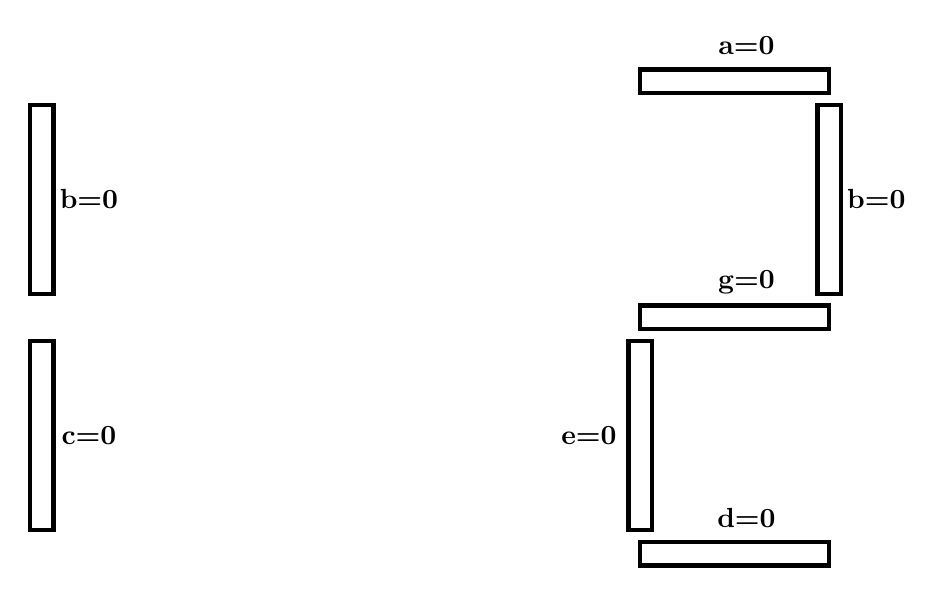
\begin{tikzpicture}
  [
    scale=1,
    >=stealth,
    point/.style = {draw, circle,  fill = black, inner sep = 0.5pt},
    dot/.style   = {draw, circle,  fill = black, inner sep = .2pt},
  ]

%Vertices of the main display rectangle
\def \xmin{0}
\def \xmax{6}
\def \ymin{0}
\def \ymax{-9}

%Number of pins on a side
\def \n{5}
\def \k{1.6}

%Define height of pins and their separation
\def \height{2}
\pgfmathsetmacro{\wid}{(\xmax-\xmin)/(\n-1)}

%Defining y axis divisions
\pgfmathsetmacro{\ywid}{(\ymin-\ymax)/(\n-2)}

%Drawing 1
\foreach [count=\i] \j in {\textbf{b=0},\textbf{c=0}}
{            
\draw[ultra thick] (\xmin+2.6*\wid,{\ymin-(\i+0.35)*\ywid } ) rectangle +(0.3,\k*\wid );
\node (\i) at ( \xmin + 3.1*\wid,{\ymin-(\i-0.05)*\ywid}) {\j} ;
}

%Drawing 2, scope helps create another figure by reusing the same coordinates
\begin{scope}[shift={(10,0)}]
\foreach [count=\i] \j in {\textbf{a=0},\textbf{g=0},\textbf{d=0}}
{            
\draw[ultra thick] (\xmin+1.1*\wid,{\ymin-(\i-0.5)*\ywid} ) rectangle +(\k*\wid,0.3 );
\node (\i) at ( \xmin + 2*\wid,{\ymin-(\i-0.7)*\ywid}) {\j} ;
}

\foreach [count=\i] \j in {\textbf{f},\textbf{e=0}}
{
\ifnum \i=2
            
\draw[ultra thick] (\xmin+\wid,{\ymin-(\i+0.35)*\ywid} ) rectangle +(0.3,\k*\wid );

\node (\i) at ( \xmin + \wid-0.5,{\ymin-(\i-0.05)*\ywid}) {\j} ;
\fi
}

\foreach [count=\i] \j in {\textbf{b=0},\textbf{c}}
{  
\ifnum \i = 1          
\draw[ultra thick] (\xmin+2.6*\wid,{\ymin-(\i+0.35)*\ywid } ) rectangle +(0.3,\k*\wid );
\node (\i) at ( \xmin + 3.1*\wid,{\ymin-(\i-0.05)*\ywid}) {\j} ;
\fi
}
  \end{scope}

%
\end{tikzpicture}
